% Source: graduate-coursework/Research/Intro_to_Agents/handouts/Part2_Agent_Foundations.tex

\documentclass[border=4pt]{standalone}
\usepackage{amsmath}
\usepackage{amssymb}
\usepackage{tikz}
\usepackage{xcolor}
\usetikzlibrary{shapes.geometric, arrows.meta, positioning, fit, calc, backgrounds}

\definecolor{UofSCGarnet}{HTML}{73000a}
\definecolor{UofSCBlack}{HTML}{000000}
\definecolor{UofSCWhite}{HTML}{ffffff}
\definecolor{UofSCAtlantic}{HTML}{466A9F}
\definecolor{UofSCCongaree}{HTML}{1F414D}
\definecolor{UofSCRose}{HTML}{CC2E40}
\definecolor{UofSCHorseshoe}{HTML}{65780B}
\definecolor{UofSCGrass}{HTML}{CED318}
\definecolor{UofSCHoneycomb}{HTML}{A49137}
\definecolor{UofSCDarkGarnet}{HTML}{570008}
\definecolor{UofSCAzalea}{HTML}{844247}
\definecolor{UofSC90Black}{HTML}{363636}
\definecolor{UofSC70Black}{HTML}{5C5C5C}
\definecolor{UofSC50Black}{HTML}{A2A2A2}
\definecolor{UofSCWarmGrey}{HTML}{676156}
\definecolor{UofSCSandstorm}{HTML}{FFF2E3}

\tikzset{
    % Box styles with sharp corners
    component/.style={
        rectangle,
        draw=UofSCBlack,
        fill=UofSCWhite,
        thick,
        minimum width=3cm,
        minimum height=1cm,
        align=center,
        font=\small
    },
    component garnet/.style={
        component,
        fill=UofSCGarnet!10,
        draw=UofSCGarnet,
        thick
    },
    component atlantic/.style={
        component,
        fill=UofSCAtlantic!10,
        draw=UofSCAtlantic,
        thick
    },
    component congaree/.style={
        component,
        fill=UofSCCongaree!10,
        draw=UofSCCongaree,
        thick
    },
    loop node/.style={
        rectangle,
        draw=UofSCGarnet,
        fill=UofSCGarnet!15,
        thick,
        minimum width=2.5cm,
        minimum height=1.2cm,
        align=center,
        font=\footnotesize\bfseries
    },
    decision/.style={
        diamond,
        draw=UofSCBlack,
        fill=UofSCHoneycomb!20,
        thick,
        minimum width=2cm,
        minimum height=1.5cm,
        align=center,
        font=\footnotesize,
        aspect=2
    },
    arrow style/.style={
        ->,
        >=Stealth,
        thick,
        UofSCBlack
    },
    biarrow style/.style={
        <->,
        >=Stealth,
        thick,
        UofSCBlack
    }
}

\begin{document}
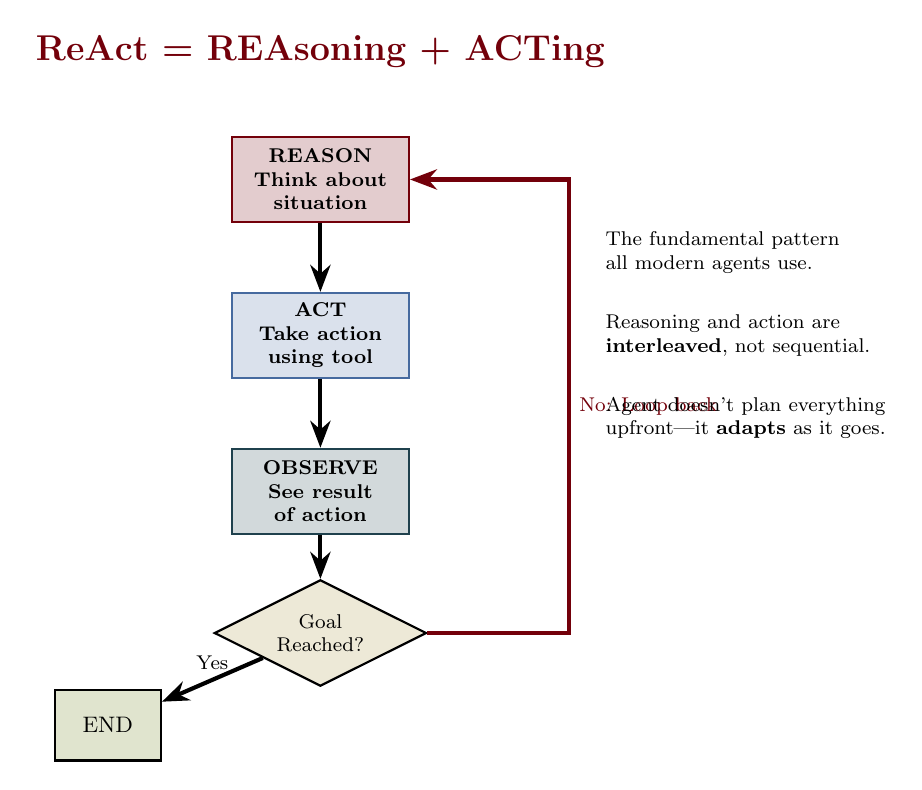
\begin{tikzpicture}[scale=0.9, transform shape]
        % Title
        \node[font=\Large\bfseries, text=UofSCGarnet] at (0, 4) {ReAct = REAsoning + ACTing};

        % REASON node
        \node[loop node, fill=UofSCGarnet!20] (reason) at (0, 2.2) {
            \textbf{REASON}\\
            Think about\\situation
        };

        % ACT node
        \node[loop node, fill=UofSCAtlantic!20, draw=UofSCAtlantic] (act) at (0, 0) {
            \textbf{ACT}\\
            Take action\\using tool
        };

        % OBSERVE node
        \node[loop node, fill=UofSCCongaree!20, draw=UofSCCongaree] (observe) at (0, -2.2) {
            \textbf{OBSERVE}\\
            See result\\of action
        };

        % Decision
        \node[decision, minimum width=2.5cm] (decision) at (0, -4.2) {Goal\\Reached?};

        % End node
        \node[component, fill=UofSCHorseshoe!20, minimum width=1.5cm] (end) at (-3, -5.5) {END};

        % Arrows
        \draw[arrow style, line width=1.5pt] (reason) -- (act);
        \draw[arrow style, line width=1.5pt] (act) -- (observe);
        \draw[arrow style, line width=1.5pt] (observe) -- (decision);
        \draw[arrow style, line width=1.5pt] (decision) -- node[above, font=\footnotesize] {Yes} (end);

        % Loop back arrow
        \draw[arrow style, line width=1.5pt, UofSCGarnet] (decision.east) -- ++(2,0) |- node[right, font=\footnotesize, pos=0.25] {No: Loop back} (reason.east);

        % Side explanation
        \node[align=left, font=\footnotesize] at (6, 0) {
            The fundamental pattern\\
            all modern agents use.\\[0.5cm]
            Reasoning and action are\\
            \textbf{interleaved}, not sequential.\\[0.5cm]
            Agent doesn't plan everything\\
            upfront---it \textbf{adapts} as it goes.
        };
    \end{tikzpicture}
\end{document}
